\begin{abstract}
Audio language models now grade spoken answers directly: automated oral
exams, AI interview screening, and speech leaderboards all use an
audio-input model as the judge, and all of them assume the judge scores what
was said, not how it sounded. We test that assumption three ways: a
text-to-speech audit that holds 24 interview answers fixed while varying
accent and gender (192 clips, three judges from two vendor families), a
replication battery that re-renders the same design with six additional
voices and a decomposed rubric, and a real-speech arm built from L2-ARCTIC
(24 speakers, six first languages) against matched native recordings. The
audit initially produced a headline: Gemini 3.1 Pro scored Indian-accented
answers 2.5 points lower than the identical American-accented answer
($p=0.005$), localized to the acoustic channel by an accent-by-grading-mode
interaction ($-6.04$ versus own-transcript grading, $p=4\times10^{-4}$). The
replication battery dissolved it. Across six additional voices the Indian
shift is $-0.76$ ($p=0.35$), with per-voice swings from $+2.08$ to $-4.58$:
the voice, not the accent, moves the score. Under a decomposed
four-dimension rubric on the original voices the penalty vanishes entirely
(all dimensions n.s.). We report this as our pre-registered discipline
requires, and we flag the general lesson: single-voice, single-rubric audit
designs, the norm in this literature, can manufacture an accent-bias
finding. On real speech the picture inverts: both Gemini judges penalise
every non-native L1, from $-4.3$ (Hindi) to $-15.7$ (Mandarin) points under
a read-aloud rubric, all $p\le4\times10^{-4}$, with close cross-judge
agreement, while the open-weight Qwen2-Audio-7B barely reacts on its
compressed scale. Twelve of these real-speech cells plus four TTS cells
survive Benjamini-Hochberg correction across all 33 accent-judge-arm tests.
What an audio judge measures depends on the voice sample, the rubric, and
the judge family; an audit that fixes all three can say more about its own
design than about the model.
\end{abstract}

\begin{figure}[t]
  \centering
  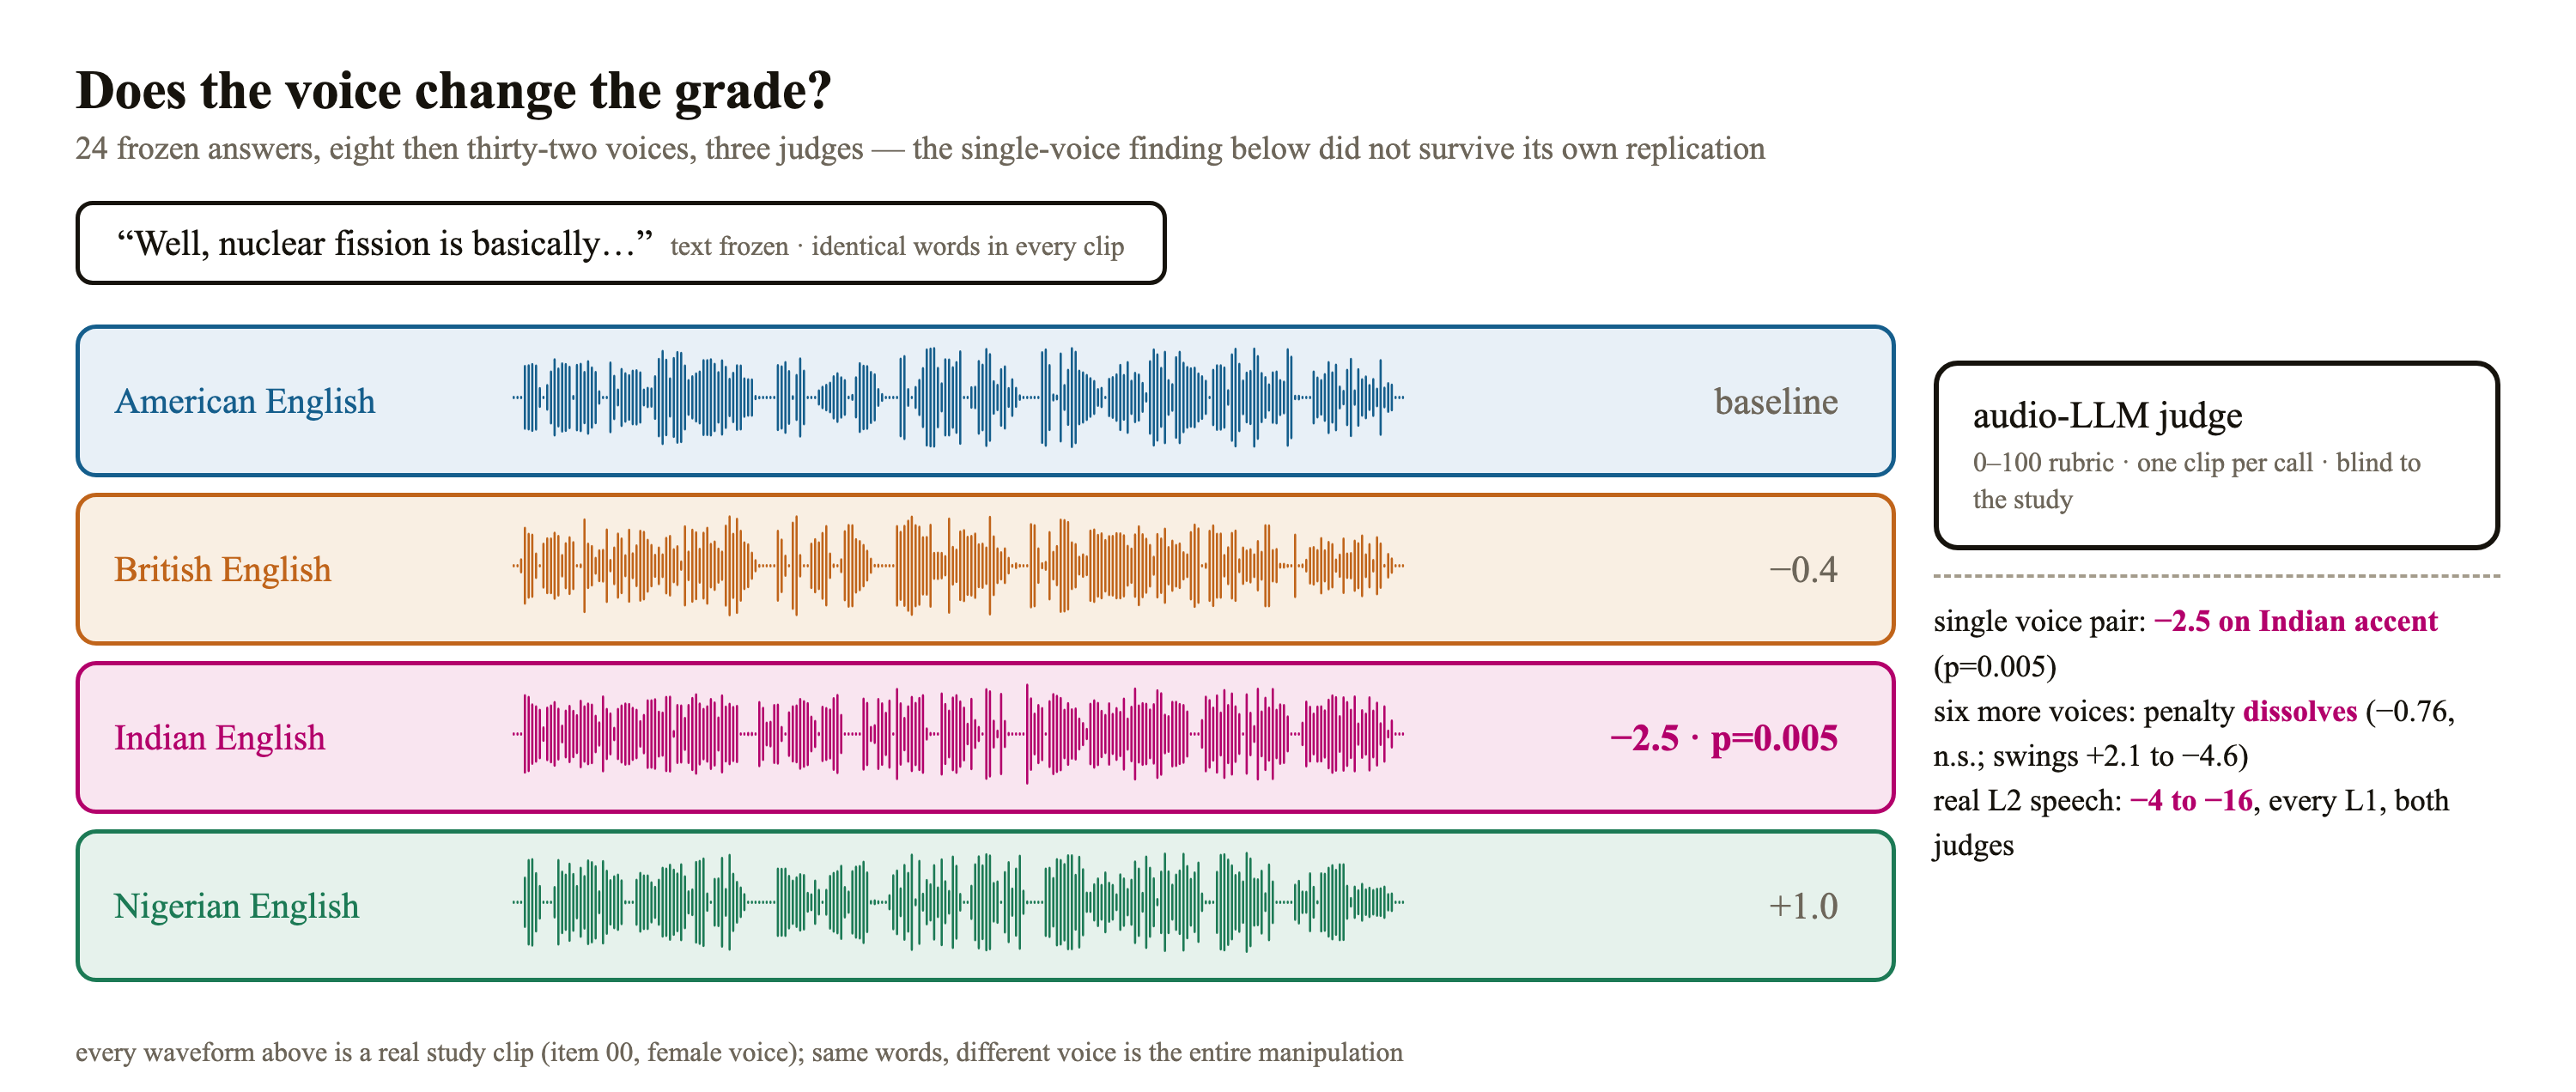
\includegraphics[width=0.88\textwidth]{assets/fig_teaser.png}
  \caption{\textbf{Study design (single-voice TTS arm).} One frozen spoken answer, rendered in four accents and two genders by TTS, scored blind by audio-input judges. Any score gap between renderings of the same item is a voice effect by construction. The $-2.5$ Indian-accent cell previewed at right is the single-voice arm's finding; \S\ref{sec:multivoice} shows it does not survive replication across voices.}
  \label{fig:teaser}
\end{figure}

\section{Introduction}

An audio language model that grades a spoken answer is being asked to do two
things at once: understand the content, and ignore everything about the
voice that carries it. Three deployed systems already depend on that second,
unstated assumption holding. Automated oral-language assessment tools grade
non-native speakers on scales that claim to measure content, not accent
\citep{ma2025assessmentof}. AI interview-screening pipelines already
process hundreds of thousands of real candidate interviews with an
LLM-as-judge step in the loop \citep{allbert2025evaluatingsp}, on top of a
pre-LLM fairness literature that already catalogued bias sources in
automated video interviews \citep{booth2023integratingp}. Speech
leaderboards increasingly use an audio-capable model, rather than a human
panel, to rank system outputs \citep{manakul2025audiojudgeun}. None of these
deployments has been checked against the one manipulation that would prove
or disprove the assumption directly: holding what is said perfectly fixed,
and changing only who appears to be saying it.

We ran that check, and this paper reports what happened when we then subjected
our own result to the replication battery a sceptical reviewer would demand.
The first arm authors 24 short answers once, freezes the text, and renders
each answer in four accents and two speaker genders with a single
text-to-speech voice pair, the standard design in this literature. It
produced a clean, significant, channel-localized accent penalty under one
judge. The second arm re-rendered the same design with six additional voices
and a decomposed rubric, and the penalty dissolved: what looked like an
accent effect was a property of one voice pair under one rubric shape. The
third arm replaced synthesis with real speech, 24 L2-ARCTIC speakers against
matched native recordings, where both Gemini judges penalise every
non-native first language, heavily, consistently, and in close agreement
with each other.

This paper makes five contributions.
\begin{enumerate}
\item A three-arm causal audit design, single-voice TTS, multi-voice TTS
replication, and real speech, that puts an audio-input model in the grader
role with the evaluee's voice as the manipulated variable
(Section~\ref{sec:method}).
\item A cautionary methods finding: a single-voice, single-rubric audit
produced a significant, multiple-comparison-surviving,
channel-localized ``accent bias'' that did not survive voice replication or
rubric decomposition (Section~\ref{sec:multivoice}). Single-voice designs
are the norm in the work we review; the failure mode generalizes.
\item A decomposition design with explicit interaction tests that localizes
the (voice-level) penalty to the acoustic channel: grading the same audio
from a transcript removes it ($-6.04$ interaction, $p=4\times10^{-4}$;
Section~\ref{sec:decomp}).
\item A real-speech arm showing large, cross-judge-consistent penalties for
all six non-native L1s under a read-aloud rubric, with a stable per-L1
gradient, alongside a third judge family that barely reacts
(Section~\ref{sec:realspeech}).
\item A delivery-perturbation battery, filled pauses, speaking rate,
telephone-bandwidth audio, and background noise, tested under both a neutral
rubric and an explicit ignore-delivery instruction, null at this sample size
(Section~\ref{sec:delivery}).
\end{enumerate}

\section{What Was Known and What Is New}

The premise that audio-language-model judges carry biases is not new. What
is new is which bias, in which role, and what a replication battery does to
it.

\textbf{AudioJudge} \citep{manakul2025audiojudgeun} establishes that
large audio models can act as judges of speech, and catalogs verbosity and
position bias in that role. It never varies the identity of the speaker
being judged; its evaluees are text-to-speech systems, not people.

\textbf{The Voice Behind the Words} \citep{satish2026thevoicebehi}, and its
companion study using the same cohort and an explicitly judge-free protocol
\citep{satish2026fromseeingit}, are the closest papers by topic. It varies the accent and gender of a
\emph{question-asker} across 2,880 controlled interactions and finds that a
SpeechLLM's own reply is rated less helpful for some accents. But the judge
in that paper is explicitly text-only and voice-blind: it reads only the
assistant's written reply, never the audio. It cannot show, and does not
claim, that an audio-input judge's score of an evaluee's own answer moves
with that evaluee's voice, which is the question this paper asks.

\textbf{BiasInEar} \citep{wei2026biasintheear} varies the voice of a spoken
multiple-choice question and measures whether the model's own answer choice
changes. The model there is the test-taker, not a judge.
\textbf{ParaPairAudioBench} \citep{jeon2026parapairaudi} puts an audio
model in the judge role and tests whether it can detect paralinguistic
differences when told to look for them, the inverse of asking whether they
leak into an unrelated content score unprompted.
\textbf{Bias Analysis of L2 Speaking Assessment Systems}
\citep{labroo2026biasanalysis} audits a real speaking-assessment grader for
encoded speaker attributes, but representationally, on naturally varying
speakers, not through a controlled same-content voice swap.

What remained uncovered, and is the subject of this paper, is the exact
intersection: an audio-input model in the grader role, the evaluee's own
voice identity as a randomized treatment, and a content score as the
outcome, with the text held identical across every condition.

Three adjacent clusters do not close the gap: judge-construction work
without a bias axis \citep{wang2025speechllmasj,zhang2026jastinaligni,
chen2025audiolargela,park2026auditingprot,chiang2025audioawarela,
liu2025vocalbenchdf,takagi2026investigatin}; advisor-role work measuring
the model's own response, not a grade \citep{wu2025evaluatingbi,
lin2026vibevoiceind,satish2025speakyourmin,satish2025dobiasbenchm,
choi2025acousticbase}; and observational audits of deployed L2 grading
\citep{uehara2026interpretabl,ginjala2026doLLMdecoders,koenecke2020racial}.
\citet{miller2026doaudiolangu} comes closest procedurally, holding a
transcript fixed while varying affect to test evidence use, but manipulates
delivery, not demographic identity. TTS-instrument validity work
\citep{zhong2025pairwiseeval,huang2026codecmosacce,xinyuan2025scalablecont,
yang2025positiontowa,ren2026mosbiasfromh} informs our manipulation checks;
our multivoice result (\S\ref{sec:multivoice}) is itself evidence for that
literature's central worry. \citet{wang2026priorongevidence} uses the same
real-speech corpus we use as our causal anchor, for a diagnostic-feedback
task rather than content grading. The human-listener precedent predates
audio language models: \citet{kang2009reverse} show identical recorded
speech is rated less comprehensible under a different apparent speaker
identity, the causal logic we apply to an artificial judge.

\textbf{Significance.} If a judge's score of a spoken answer depends on the
speaker's voice, every deployed pipeline above is partly scoring the speaker
rather than the answer. Our results sharpen this in two directions at once:
audits using one synthetic voice per condition can \emph{overstate} accent
effects (ours did), while on real speech the voice sensitivity of two
production judges is large, consistent, and graded by first language.

\section{Method}
\label{sec:method}

\subsection{Answer Bank}

We authored 24 interview-style question-and-answer pairs across ten everyday
domains, using a frozen text model, each targeting a medium quality band so
a judge has headroom to move the score. A first calibration failed
instructively: ``incomplete or shallow'' answers scored a ceiling-level mean
of 94.3/100 under a real audio judge. A rewritten prompt requiring
checkable weaknesses, validated on five test answers (35 to 65),
regenerated the bank at mean 61.3 (sd 17.0, range 20 to 90 under Gemini 3.6
Flash), the distribution used throughout.

\subsection{Axis A: Accent and Gender, Single-Voice Arm}

Each answer was rendered with \texttt{gemini-3.1-flash-tts-preview} in four
accents (American, British, Indian, Nigerian English) crossed with two
voices (one male, one female: the Charon/Kore pair), producing 192 clips.
Accent is a natural-language style instruction to the TTS engine. An 8-clip
manipulation check preceded generation: a blind classifier judge identified
the intended accent and gender in 8 of 8 clips at high stated confidence.
Every clip was loudness-normalized (\texttt{ffmpeg loudnorm}) and resampled
to 16kHz.

\subsection{Axis A$^{+}$: Multi-Voice Replication and Decomposed Rubric}
\label{sec:method-multivoice}

Because a single voice per accent-gender cell aliases accent with everything
else that voice carries, we re-rendered a 12-item subset in all four accents
with six additional prebuilt voices (three per gender: Puck, Fenrir, Orus;
Aoede, Leda, Zephyr), producing 288 further clips judged identically by both
Gemini judges. Separately, we re-judged the full original 192-clip arm under
a decomposed rubric that scores correctness, completeness, helpfulness, and
clarity from 0 to 25 each, rather than one 0 to 100 score, to test whether
the rubric's shape carries part of the effect.

\subsection{Axis A$'$: Real Speech (L2-ARCTIC $\times$ CMU ARCTIC)}
\label{sec:method-realspeech}

The real-speech arm uses L2-ARCTIC \citep{zhao2018l2arctic}: 24 non-native
English speakers, two male and two female for each of six first languages
(Arabic, Hindi, Korean, Mandarin, Spanish, Vietnamese), reading the same
prompt sentences as the native CMU ARCTIC voices. We selected eight
sentences verified present for all 24 L2 speakers and all six native
reference voices (bdl, rms, jmk, awb male; slt, clb female), 240 clips
total, resampled to a common 16kHz and loudness-normalized identically to
the TTS arms, since the two corpora ship at different sample rates. Because
ARCTIC sentences are generic prompts rather than domain answers, the rubric
for this arm scores the \emph{reading}: clarity, fluency, and how
professional it sounds, 0 to 100 (verbatim in
Appendix~\ref{app:prompts}). This is a delivery rubric by design; the arm
measures how strongly judges respond to non-native speech, not content bias.

\subsection{Axis B: Delivery Perturbations}

Using one fixed voice (American female), we generated five perturbations of
each answer: filled pauses, slowed (0.85$\times$) and sped (1.25$\times$)
renderings, an 8kHz telephone codec, and pink noise at 10dB SNR. Every
perturbed clip passed a word-error-rate neutrality gate ($\le$5\% WER
against the frozen text); 5 of 120 conditions failed and were excluded
(after a stricter transcription prompt eliminated 28 spurious failures
caused by the transcriber inventing content, not mis-hearing it). Both
prompt arms, neutral and explicit ignore-delivery, ran on the 139 surviving
clips.

\subsection{Judges, Protocol, and Analysis}

Three judges scored Axis A: \texttt{gemini-3.6-flash} and
\texttt{gemini-3.1-pro-preview} through the API at temperature zero, one
clip per call, randomized order, never told the study concerns voice; and
the open-weight \texttt{Qwen2-Audio-7B-Instruct} on a single A10G GPU with
greedy decoding. The rubric asks for one 0 to 100 score (correctness,
completeness, helpfulness, clarity) plus a one-sentence reason as JSON. The
Gemini judges also scored the multivoice, decomposition, delivery, and
real-speech arms; Qwen2-Audio scored Axis A and the real-speech arm. The
unit of analysis is the within-item paired difference against the matched
reference (gender-matched American rendering for TTS arms; gender-matched
native mean for real speech), with bootstrap 95\% CIs (10{,}000 resamples),
two-sided sign-flip permutation tests (20{,}000 permutations), and paired
$d_z$. Every number below is read from scripted analysis passes over the raw
logs, which ship with the paper.

\section{Results}
\label{sec:results}

\subsection{The Single-Voice Arm Produces a Clean Finding}

Table~\ref{tab:axisa} and Figure~\ref{fig:forest} report the single-voice
arm. Gemini 3.1 Pro shows one shift that clears our threshold:
Indian-accented answers score 2.5 points lower than the identical
American-accented answer ($p=0.005$, $d_z=-0.44$), while the same comparison
under Gemini 3.6 Flash is indistinguishable from zero ($-0.04$, $p=1.0$).
The third family reverses the sign: Qwen2-Audio-7B scores \emph{every}
non-American accent higher (UK $+2.92$, $p=0.011$; Indian $+1.98$,
$p=0.044$; Nigerian $+2.29$, $p=0.014$; $n{=}48$ each), though its absolute
scores cluster on a coarse four-value grid around 75. The gender main
effect is not significant for either Gemini judge (Flash trends $+3.25$
toward the female voice, $p=0.12$). Taken alone, this arm tells a tidy
story: a significant, judge-specific accent penalty. The next subsection is
why we no longer tell it.

\begin{table}[t]
\centering
\small
\caption{Single-voice TTS arm: accent shift versus the gender-matched American baseline, three judges, $n=48$ paired comparisons per cell. Bold marks cells that survive Benjamini-Hochberg correction across all 33 accent-judge-arm tests in the paper (\S\ref{sec:realspeech}). Qwen2-Audio's absolute scores fall on a coarse four-value grid.}
\label{tab:axisa}
\begin{tabular}{lrrr}
\toprule
Accent & Mean shift & 95\% CI & $p$ \\
\midrule
\multicolumn{4}{l}{\emph{Gemini 3.1 Pro}} \\
UK      & $-0.42$ & [$-2.08$, $1.25$]  & 0.73 \\
Indian  & \textbf{$-2.50$} & [$-4.06$, $-0.94$] & \textbf{0.005} \\
Nigerian& $+1.04$ & [$-0.52$, $2.60$]  & 0.26 \\
\midrule
\multicolumn{4}{l}{\emph{Gemini 3.6 Flash}} \\
UK      & $-1.08$ & [$-3.90$, $1.92$]  & 0.49 \\
Indian  & $-0.04$ & [$-2.85$, $2.73$]  & 1.00 \\
Nigerian& $+0.23$ & [$-2.60$, $3.08$]  & 0.89 \\
\midrule
\multicolumn{4}{l}{\emph{Qwen2-Audio-7B (open weight)}} \\
UK      & \textbf{$+2.92$} & [$+0.94$, $+5.00$] & \textbf{0.011} \\
Indian  & $+1.98$ & [$+0.21$, $+3.75$] & 0.044 \\
Nigerian& \textbf{$+2.29$} & [$+0.73$, $+4.06$] & \textbf{0.014} \\
\bottomrule
\end{tabular}
\end{table}

\begin{figure}[t]
\centering
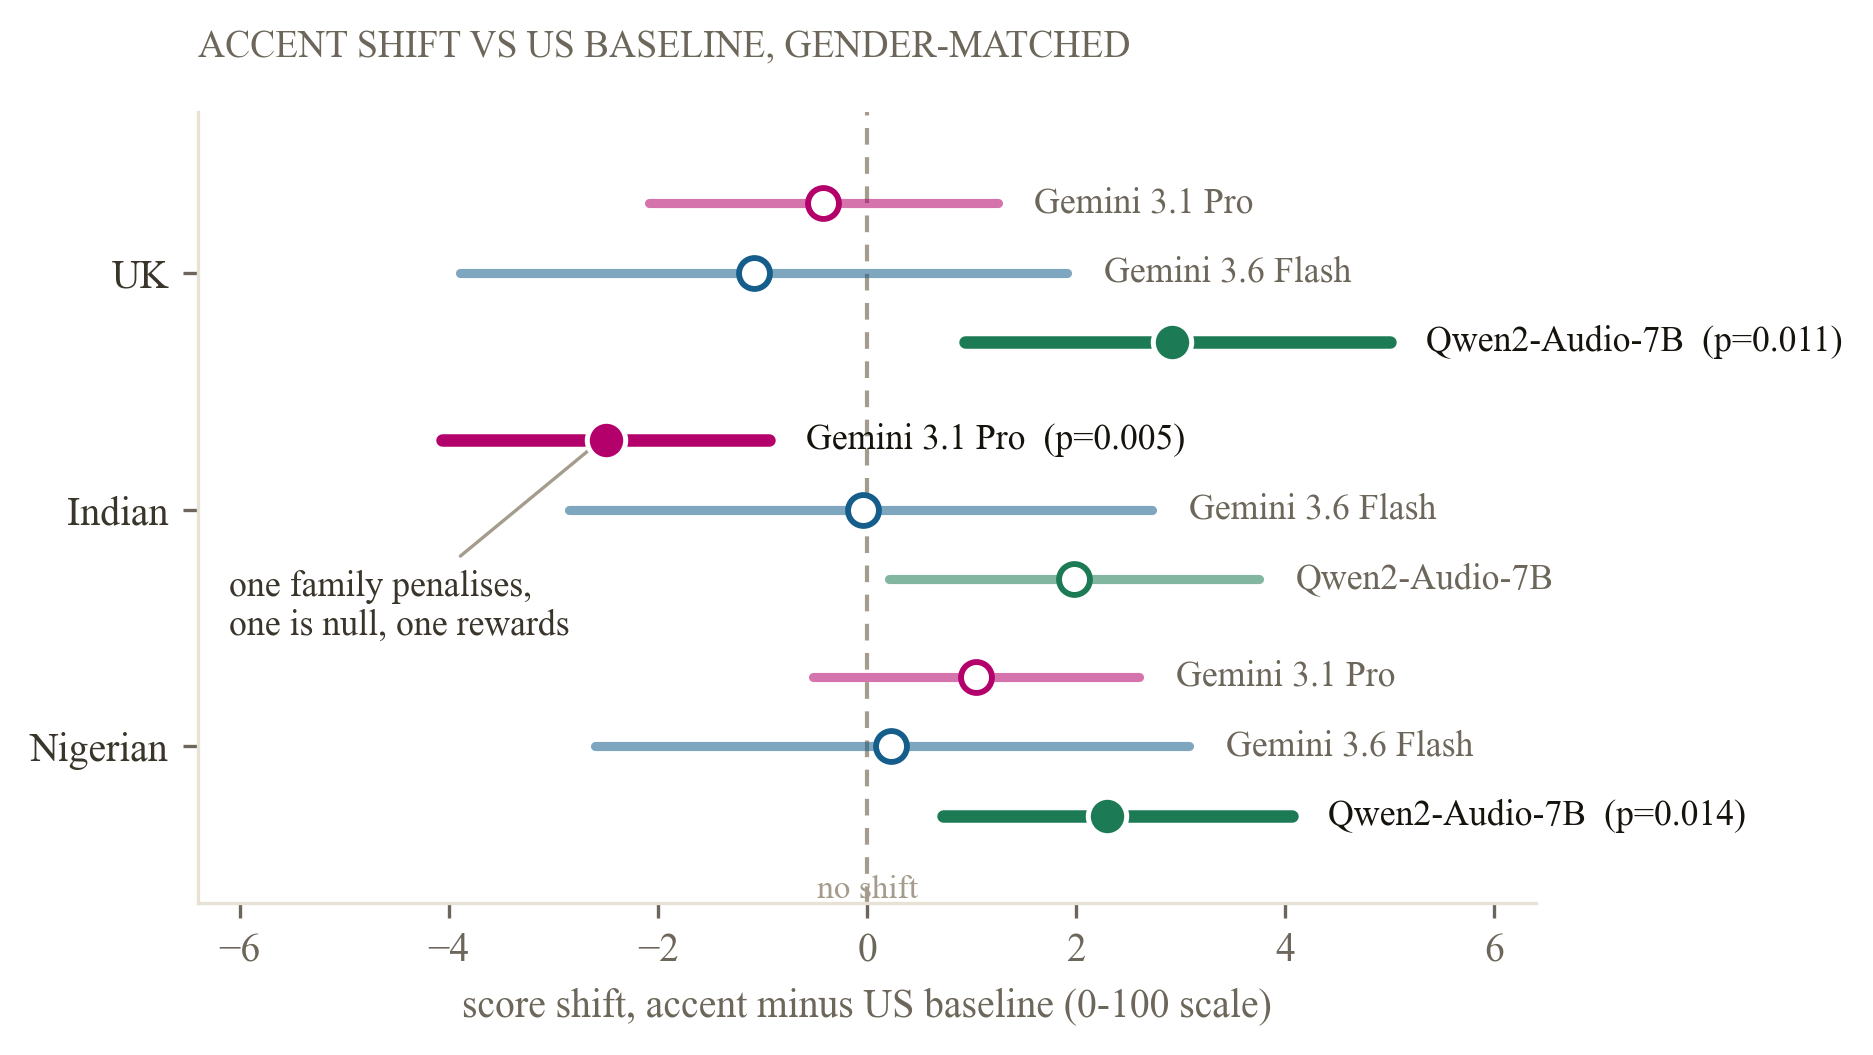
\includegraphics[width=0.78\textwidth]{assets/figure1_accent_forest.png}
\caption{Single-voice TTS arm: score shift by accent and judge, 95\%
bootstrap confidence intervals, $n=48$ paired comparisons per interval.
Right of the dashed line means the accent scored higher than the American
baseline. Filled markers survive the joint Benjamini-Hochberg correction of
\S\ref{sec:realspeech}.}
\label{fig:forest}
\end{figure}

\subsection{The Finding Does Not Survive Its Replication Battery}
\label{sec:multivoice}

We pre-registered the direction of the accent effect before collecting any
data, and pre-registration discipline cuts both ways: it obliges us to
report reversals on replication as plainly as confirmations. Both
replications reversed.

\textbf{Six more voices.} Across six additional voices rendering the same
items and accent instructions (Table~\ref{tab:multivoice},
Figure~\ref{fig:multivoice}), Pro's Indian shift is $-0.76$
(CI $[-2.22, +0.69]$, $p=0.35$, $n{=}72$), and the per-voice means swing
from $+2.08$ (Fenrir) to $-4.58$ (Zephyr). The original Charon/Kore pair's
$-2.50$ sits inside that swing, not outside it: the voice, not the accent,
moves the score. Flash is equally unstable across voices (Indian $+0.11$,
$p=0.95$; per-voice $-2.67$ to $+4.17$), and its multivoice Nigerian cell
comes out significantly \emph{negative} ($-3.22$, $p=0.0042$) where its
single-voice Nigerian trend was positive, a sign flip across voice samples
within one judge.

\textbf{A different rubric shape.} Re-judging the original 192 clips under
the decomposed four-dimension rubric, Pro's Indian-vs-American shift
vanishes: correctness $-0.15$ ($p=0.66$), completeness $-0.17$ ($p=0.56$),
helpfulness $+0.21$ ($p=0.46$), clarity $-0.23$ ($p=0.48$), total $-0.33$
on the 100-point equivalent ($n{=}48$). The same clips that produce $-2.50$
under a single holistic score produce nothing under sub-scores.

A finding can survive multiple-comparison correction (the $-2.50$ cell does,
even in the joint 33-test family below) and still fail replication:
correction controls false positives within a design, not the design's own
aliasing. The lesson is uncomfortable for this literature: a one-voice,
one-rubric audit can manufacture a clean, significant, channel-localized
``bias'' that is really a statement about that voice under that rubric.

\begin{table}[t]
\centering
\small
\caption{Multi-voice replication: accent shift versus the gender-matched American baseline across six new voices, $n=72$ paired comparisons per cell (12 items $\times$ 6 voices). Bold: survives the joint BH correction.}
\label{tab:multivoice}
\begin{tabular}{lrrr}
\toprule
Accent & Mean shift & 95\% CI & $p$ \\
\midrule
\multicolumn{4}{l}{\emph{Gemini 3.1 Pro}} \\
UK      & $+0.90$ & [$-0.69$, $+2.57$] & 0.32 \\
Indian  & $-0.76$ & [$-2.22$, $+0.69$] & 0.35 \\
Nigerian& $+1.53$ & [$+0.14$, $+2.92$] & 0.043 \\
\midrule
\multicolumn{4}{l}{\emph{Gemini 3.6 Flash}} \\
UK      & $-1.81$ & [$-4.03$, $+0.42$] & 0.12 \\
Indian  & $+0.11$ & [$-2.11$, $+2.33$] & 0.95 \\
Nigerian& \textbf{$-3.22$} & [$-5.38$, $-1.14$] & \textbf{0.0042} \\
\bottomrule
\end{tabular}
\end{table}

\begin{figure}[t]
  \centering
  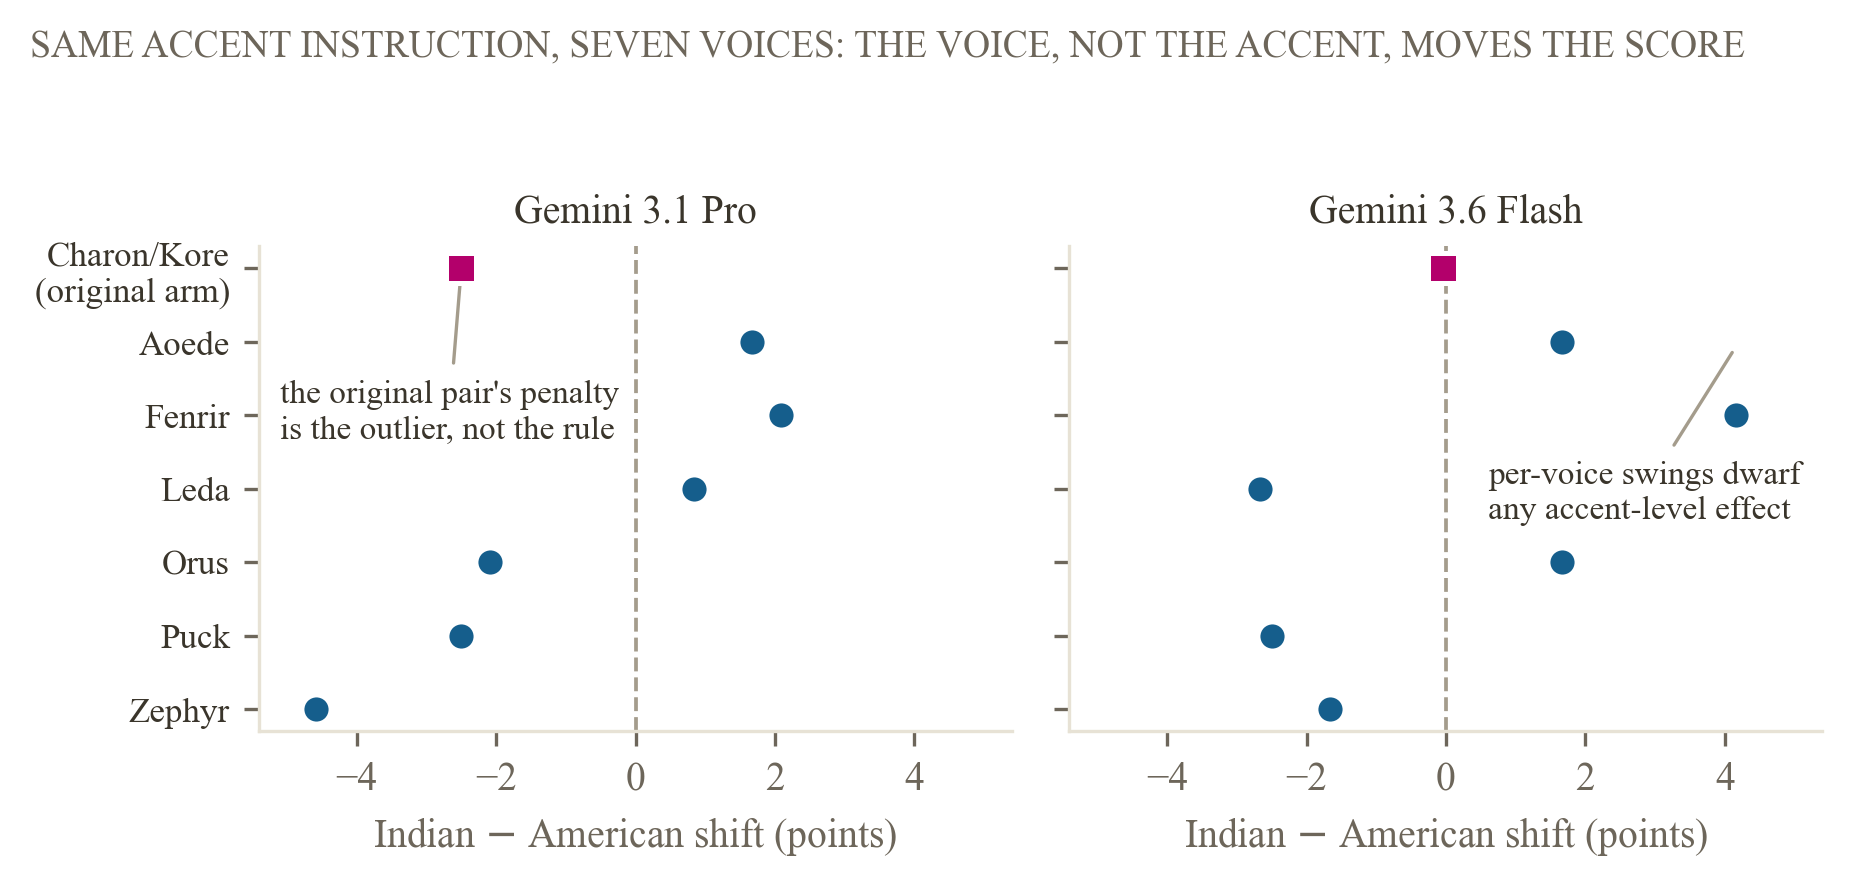
\includegraphics[width=0.88\textwidth]{assets/figure4_multivoice.png}
  \caption{\textbf{The Indian-accent shift is a property of the voice.} Per-voice Indian-minus-American mean shift ($n{=}12$ item-gender pairs per voice; original arm $n{=}48$). The original pair's penalty sits inside the per-voice swing, not outside it.}
  \label{fig:multivoice}
\end{figure}

\subsection{Where the Voice-Level Penalty Lives}
\label{sec:decomp}

For the original voice pair, where the penalty exists, the decomposition arm
grades the same content three ways (Table~\ref{tab:decomp},
Figure~\ref{fig:decomp}): end-to-end audio $-2.50$, the judge's own
transcript of the same audio $+1.88$, the frozen gold transcript $-0.83$.
Because a difference in significance is not a significant difference, we
test the accent-by-mode interaction directly: the audio-mode shift differs
from the own-transcript shift by $-6.04$ points (CI $[-8.5, -3.5]$,
$p=4\times10^{-4}$, $n{=}24$) and from the gold-transcript shift by $-3.33$
($[-5.8, -0.8]$, $p=0.028$). Whatever this judge penalises about this voice
pair lives in the acoustic channel and does not survive transcription. The
gold-transcript arm is a sanity check rather than evidence, since identical
transcripts must tie for a deterministic judge; the informative contrast is
audio versus the judge's own transcript. Flash, with no audio-mode effect to
decompose, shows nothing informative in either transcript mode ($-4.25$,
$p=0.17$; $+0.83$, $p=0.36$). Transcript-first grading thus remains a tested
mitigation, but for a voice-level artifact, which reframes what it
mitigates: it removes whatever the acoustic channel carries, legitimate or
not.

\begin{figure}[t]
  \centering
  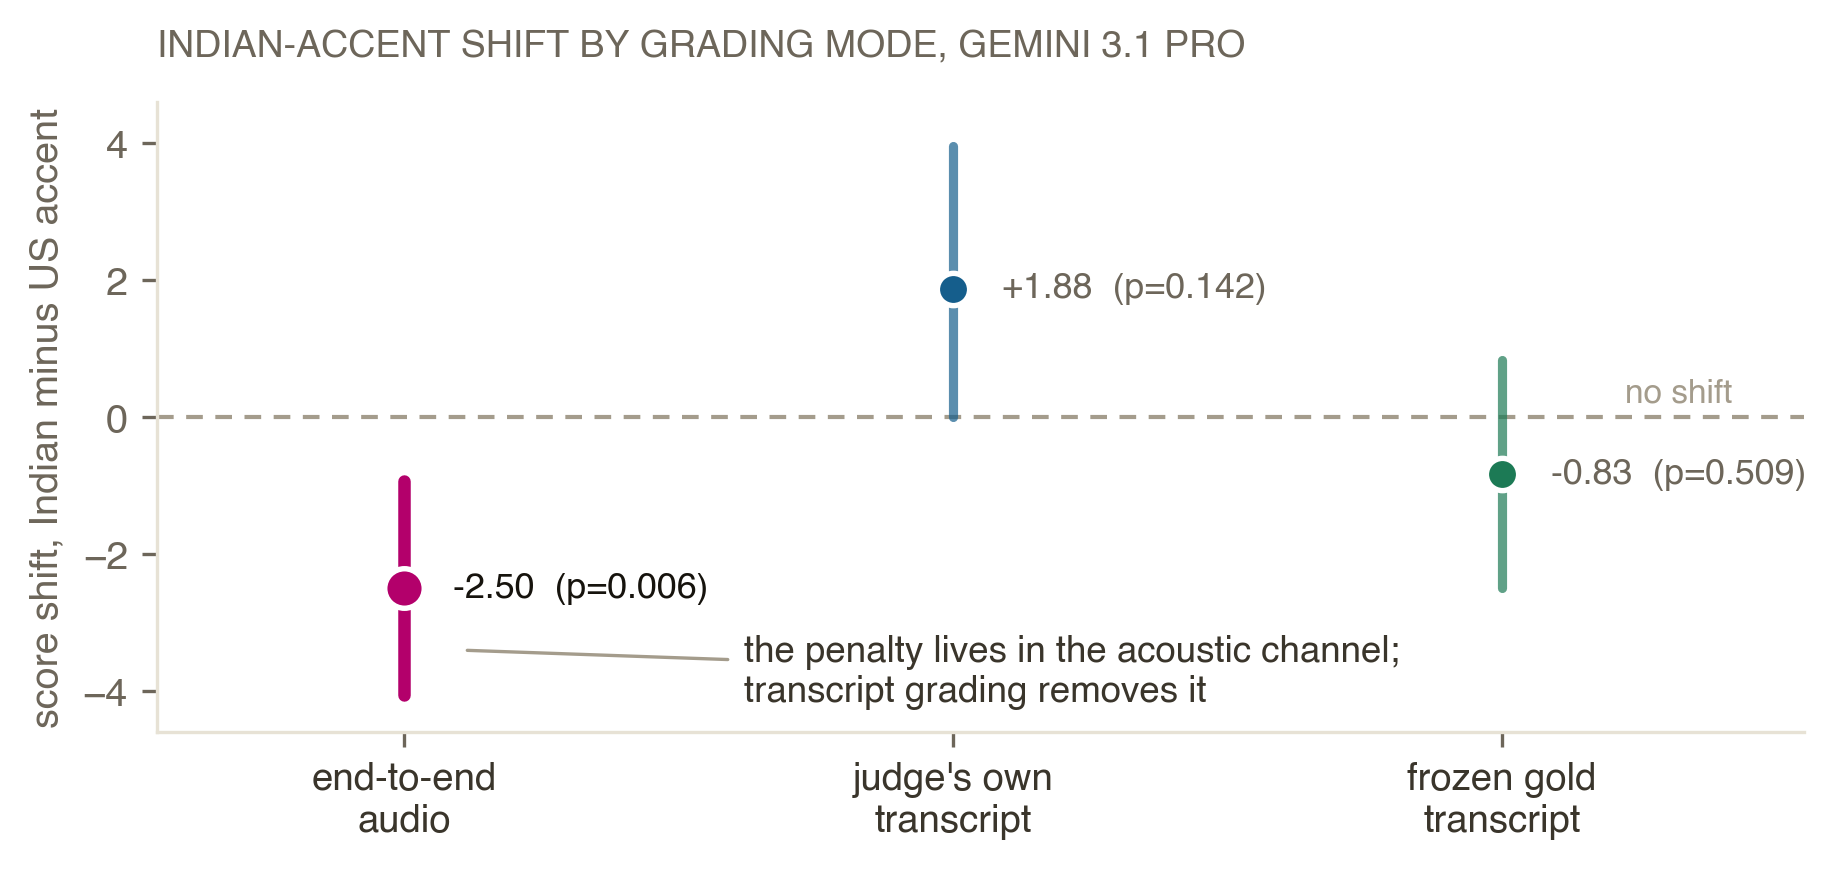
\includegraphics[width=0.72\textwidth]{assets/figure2_decomposition.png}
  \caption{\textbf{The voice-level penalty lives in the acoustic channel.} The Gemini 3.1 Pro Indian-accent shift (original voice pair) under three grading modes; interaction tests in \S\ref{sec:decomp}.}
  \label{fig:decomp}
\end{figure}

\begin{table}[t]
\centering
\small
\caption{Decomposition of the Indian-accent shift by grading mode, Gemini
3.1 Pro, original voice pair. Transcript modes: $n{=}24$ paired comparisons.
The audio row reproduces the Table~\ref{tab:axisa} cell ($n{=}48$);
interaction tests use the 24 pairs common to all modes.}
\label{tab:decomp}
\begin{tabular}{lrrr}
\toprule
Mode & Mean shift & 95\% CI & $p$ \\
\midrule
Audio (from Table~\ref{tab:axisa}) & $-2.50$ & [$-4.06$, $-0.94$] & 0.005 \\
Own transcript   & $+1.88$ & [$0.00$, $3.96$]   & 0.14 \\
Gold transcript  & $-0.83$ & [$-2.50$, $0.83$]  & 0.51 \\
\bottomrule
\end{tabular}
\end{table}

\subsection{Real Speech: Large, Consistent, and Graded by First Language}
\label{sec:realspeech}

On the 240 real recordings, both Gemini judges penalise every non-native L1
relative to gender-matched native voices reading the same sentences
(Figure~\ref{fig:l2arctic}, Table~\ref{tab:l2arctic}): under Pro, from
$-4.27$ (Hindi, $p=3\times10^{-4}$) to $-15.67$ (Mandarin, $p<10^{-4}$);
under Flash, from $-6.08$ to $-14.20$; all twelve cells
$p\le4\times10^{-4}$, $n{=}32$ per cell, four speakers per L1. The two
judges agree closely on both size and ordering (Hindi least penalised,
Mandarin and Vietnamese most), a sharp contrast to their disagreement on
the TTS arms. Qwen2-Audio, judging the identical clips, shifts by at most
$-1.25$ (all n.s.), though it compresses essentially all clips onto two
score values, so its flatness is partly an instrument property.

Two framings must be kept apart. This arm's rubric scores the
\emph{reading}, so a penalty is responsiveness to non-native delivery, not
demonstrated content bias, and real L2 speech genuinely varies in fluency.
What the arm establishes is the magnitude, consistency, and L1-gradient of
that responsiveness in production judges, and that it replicates across
speakers within each L1, which the TTS arm's effects did not across
voices.

Across all 33 accent-judge-arm tests reported in this paper,
Benjamini-Hochberg at $q=0.05$ retains 16: all twelve real-speech Gemini
cells, the single-voice Pro-Indian and Qwen UK and Nigerian cells, and the
multivoice Flash-Nigerian cell.

\begin{figure}[t]
  \centering
  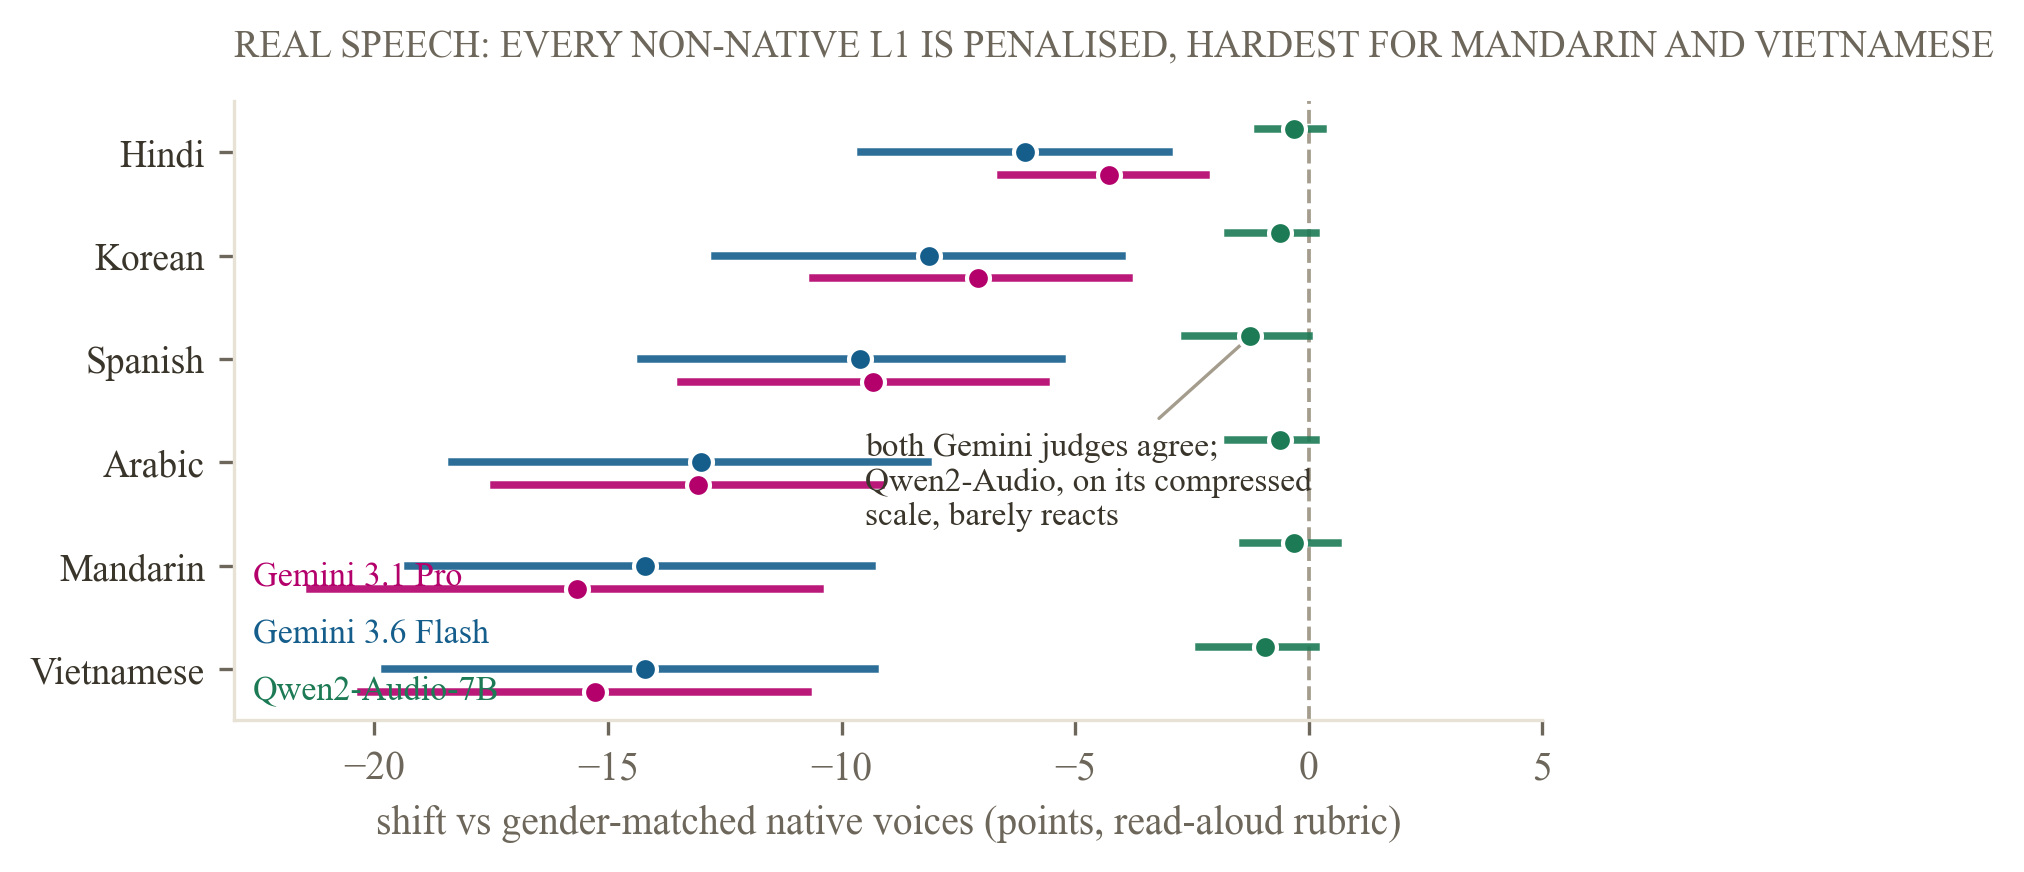
\includegraphics[width=0.85\textwidth]{assets/figure5_l2arctic.png}
  \caption{\textbf{Real speech.} Per-L1 shift versus gender-matched native voices, read-aloud rubric, 95\% bootstrap CIs, $n{=}32$ clips per cell (4 speakers $\times$ 8 sentences). Both Gemini judges agree on size and ordering; Qwen2-Audio barely reacts on its compressed scale.}
  \label{fig:l2arctic}
\end{figure}

\begin{table}[t]
\centering
\small
\caption{Real-speech arm: mean shift versus gender-matched native baseline (Pro native means 94.2/94.7 m/f; Flash 93.9/95.6), $n{=}32$ per cell. All Gemini cells survive the joint BH correction; no Qwen2-Audio cell is significant.}
\label{tab:l2arctic}
\begin{tabular}{lrrrrrr}
\toprule
 & \multicolumn{2}{c}{Gemini 3.1 Pro} & \multicolumn{2}{c}{Gemini 3.6 Flash} & \multicolumn{2}{c}{Qwen2-Audio} \\
L1 & shift & $p$ & shift & $p$ & shift & $p$ \\
\midrule
Hindi      & $-4.27$  & $3\times10^{-4}$ & $-6.08$  & $4\times10^{-4}$ & $-0.31$ & 0.75 \\
Korean     & $-7.08$  & $2\times10^{-4}$ & $-8.14$  & $2\times10^{-4}$ & $-0.62$ & 0.37 \\
Spanish    & $-9.33$  & $<10^{-4}$ & $-9.61$  & $<10^{-4}$ & $-1.25$ & 0.14 \\
Arabic     & $-13.08$ & $<10^{-4}$ & $-13.02$ & $<10^{-4}$ & $-0.62$ & 0.37 \\
Mandarin   & $-15.67$ & $<10^{-4}$ & $-14.20$ & $<10^{-4}$ & $-0.31$ & 0.75 \\
Vietnamese & $-15.27$ & $<10^{-4}$ & $-14.20$ & $<10^{-4}$ & $-0.94$ & 0.25 \\
\bottomrule
\end{tabular}
\end{table}

\subsection{Delivery (Axis B)}
\label{sec:delivery}

\begin{figure}[t]
  \centering
  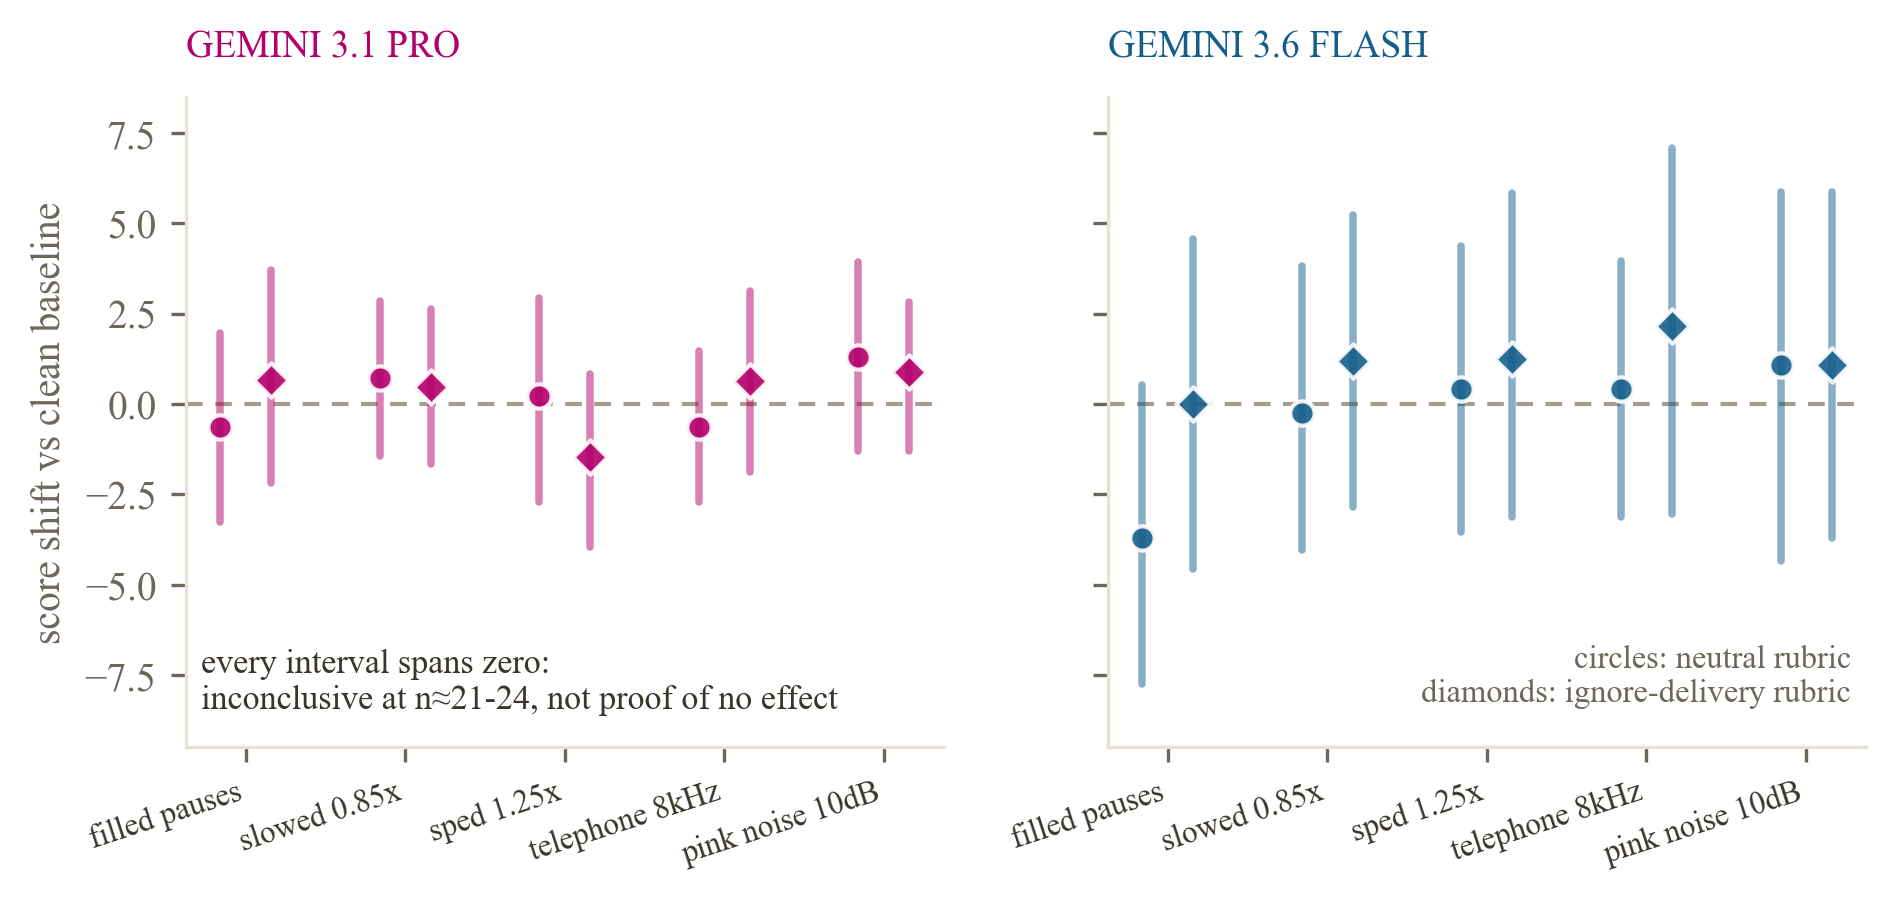
\includegraphics[width=0.9\textwidth]{assets/figure3_delivery.png}
  \caption{\textbf{Delivery perturbations: all null at this sample size.} Five perturbations, two judges, two prompt arms; every 95\% interval spans zero ($n{=}21$--$24$ per cell). Read as inconclusive, not as proof of no effect.}
  \label{fig:delivery}
\end{figure}

None of the five delivery perturbations produced a significant score shift
under either Gemini judge, under either prompt arm (all $p>0.1$,
$|d_z|<0.36$; $n$ of 21 to 24 per cell after WER exclusions). We read this
as inconclusive at this sample size, as our planning-stage power analysis
anticipated for the secondary axis, not as evidence that delivery never
leaks into content scores.

\section{Limitations}
\label{sec:limitations}

\textbf{The rubrics differ across arms by design.} The TTS arms score
content dimensions; the real-speech arm scores the reading itself, because
ARCTIC sentences carry no domain content. The real-speech penalties are
therefore delivery-responsiveness results, and their size should not be
read as content bias. A content-bearing real-speech corpus would close this
gap.

\textbf{Real-speech recording conditions are confounded with nativeness.}
The native CMU ARCTIC voices are studio recordings of experienced voice
talent; L2-ARCTIC speakers are not professional narrators. Part of the
per-L1 gradient may reflect recording and speaker professionalism rather
than accent per se. Four speakers per L1 also limits speaker-level
generality, though the within-L1 consistency across speakers and across two
judges is what the TTS arm's effects lacked.

\textbf{Sample size.} The TTS arms use 24 items under a \$20 compute
budget; the delivery nulls and the non-significant multivoice cells may be
underpowered. The multivoice arm covers 12 of the 24 items.

\textbf{Judge coverage is uneven.} Both Gemini judges scored every arm;
Qwen2-Audio scored the single-voice TTS and real-speech arms only.
Qwen2-Audio's compressed output scale (two to four distinct values) limits
what its null shifts can show. A frontier non-Google audio judge remains
untested.

\textbf{Same-family manipulation check.} The 8-clip accent-fidelity check
used a Gemini classifier on Gemini-generated audio; an independent or
human-listener check has not been run. The multivoice results reduce the
weight this check carries, since we no longer rest an accent claim on the
TTS arm.

\textbf{The noise condition is a proxy.} Pink noise at measured SNR stands
in for licensed multi-talker babble.

\section{Conclusion}

We asked whether an audio-input judge's score moves with the speaker's
voice when the words are held fixed, and the honest answer required three
designs. A single-voice audit said yes, significantly, for one judge and
one accent, localized to the acoustic channel. Six more voices said the
penalty belongs to the voice, not the accent, and a decomposed rubric made
it vanish on the original voices; we report our own headline as a
replication failure, because that is what pre-registration is for. Real
speech then said something larger: on actual non-native speakers, two
production judges penalise every first language we tested, by up to fifteen
points, consistently with each other and graded by L1, under a rubric that
scores delivery. The practitioner checklist: audit with multiple voices per condition or
real speakers, never one; treat rubric shape as a design variable; and know
that transcript-first grading removes whatever the acoustic channel
carries, a mitigation only if that is what you intend. Whether the large
real-speech penalties are calibrated to human judgment of the same
recordings is the natural next experiment.
